\documentclass[overlapped,line,final]{res}

\usepackage[main=english,spanish]{babel} % spanish Latex support
\usepackage[utf8]{inputenc} % 
\usepackage{graphicx}       % graphics support
\usepackage[T1,hyphens]{url}
\usepackage[breaklinks]{hyperref} %url hyphenation
\usepackage{microtype}
\usepackage{fontawesome5}
\usepackage{xcolor}
\usepackage{verbatim}

\definecolor{NemQLinks}{rgb}{0.1, 0.3, 0.6}

\hypersetup{
    colorlinks,
    linkcolor={red!50!black},
    citecolor={blue!50!black},
    %urlcolor={red!80!black}
    urlcolor={NemQLinks}
}


%----------------------------------------------------------
%----------------------------------------------------------header
\begin{document}

%name
\name{{\Large \bf David Toro Triana}}

\begin{resume}

%-----------------------------------------------personal info, photo

%\begin{minipage}{\linewidth}
	\begin{minipage}{0.5\linewidth}
%    		Carrera 15 \# 188-11  \newline 
    		Bogotá D.C., Colombia \newline
    		(+57) 313 255 98 64 \newline
		{\tt \href{mailto:dtorot@opensai.org}{dtorot@opensai.org}}
     	%{\tt https://opensai.org} 
	\end{minipage}
%	\begin{minipage}{0.5\linewidth}
%		\begin{center}
%			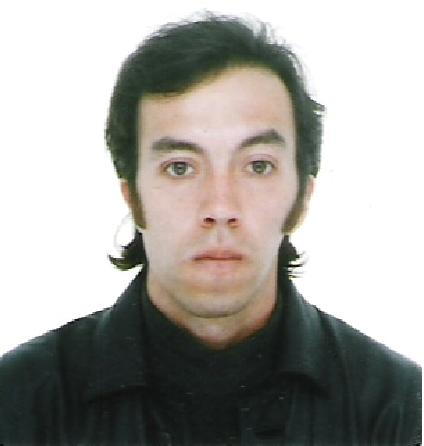
\includegraphics[bb=0 0 100 105, width=30mm,keepaspectratio]{foto.jpeg}
%\begin{center}
%	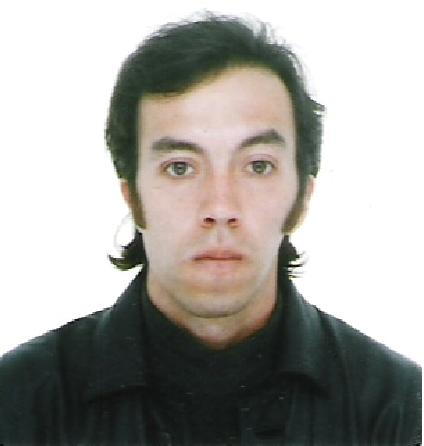
\includegraphics[width=3cm, bb=0 0 305 321]{./foto.jpeg}
%	% foto.jpeg: 424x446 pixel, 100dpi, 10.77x11.33 cm, bb=0 0 305 321
%\end{center}
%		\end{center}
%	\end{minipage}
%\end{minipage}


%----------------------------------------------------Professional Profile 
\vspace{0.5cm}
\section{\sc Professional Profile}
\vspace{0.5cm}
During the last 10 years, I have been working in the field of Web Development and GNU/Linux Systems Administration, thanks to the FLOSS ( {\em Free Libre Open Source Software } ) movement, which allowed me to research, to learn and to contribute to industry and the academy in those fields:

\vspace{2mm}
\begin{itemize}
    \item I have experience in the deployment and administration of LAMP services, in the main GNU/Linux distributions (Redhat, CentOS, Debian-Ubuntu). 

    \item Also I have worked as Frontend Developer using web standards like HTML5, CSS3 and JavaScript, CSS preprocessors (Bootstrap), using the most popular CMS's (WordPress, Joomla!).

\end{itemize}
    
	\textbf {I understand that the technology is merely a tool to get organizational goals. From a multicultural environments and goal-oriented leadership, I like to build and maintain productive relationships with clients and colleagues, to gathering, assessing and analysing customer needs, translating business requirements in solution design and effective customer experience.}

%-----------------------------------------------------Projects
% \vspace{1cm}
\vspace{0.5cm}
\section{\sc Projects } %-- twixt \location{} & \begin{position}
\vspace{0.5cm}
% -------------------------------------------
\title{\bf Legal Representation
	\newline \em Open Source Academic Initiative (NGO).
	\newline {\tt \url {https://opensai.org} } 
}
\employer{\em Legal Rep. (Substitute) – \bf Miguel Ángel González Garzón}
\location{\em (+57) 320 3614052 }
\dates{\bf  January 2013 - March 2022 }
\begin{position}
Legal Representation and projects management:
	\begin{itemize}
		\item \href{https://opensai.org/business}{Management of Open Source Services Brief \faIcon{external-link-alt}}
		\item Signing of the cooperation agreement with the Universidad Nacional de Colombia (Faculty of Engineering – October 2014)
		\item Development of pedagogical content and follow-up of the educational process of the \textit{Programa de Fortalecimiento de Capacidades - Formación en animación digital, 2D, 3D, StopMotion y Efectos Especiales ANIMADELAB} (Faculty of Engineering, Universidad Nacional de Colombia - 2015 - MinTIC)
		\item Learning platform (EdX) for blind people (Faculty of Engineering, Universidad Nacional de Colombia, INCI - 2015 )
		\item Signing of the cooperation agreement with the Universidad Minuto de Dios – \#OpenLAB (Faculty of Engineering – February 2017)
		\item \href{https://rea.opensai.org/}{OpenSAI-SENA-SENNOVA ReA Project \faIcon{external-link-alt}}. Development of a prototype of an augmented reality App for the Epson SmartGlass Moverio BT 300, to to help the navigation in a package store for the logistic sector (April 2018 - May 2019)
		\item Development of the Valure Web Site: \href{https://valure.com.co}{\textit{High level Agency of Consultancy, political and government issues} \faIcon{external-link-alt}} (AWS, Bitnami, internal API's integration - November 2021)
	\end{itemize}
%\end{position}
\newpage
\opening
% -------------------------------------------
%\begin{position}
\textbf{OpenSAI Teaching Experience}: the promotion, divulgation and teaching in Open Source Technologies is one of the missional functions in that \textit{NGO}. I has participated in many workshops, seminars, courses organized by them:
\begin{itemize}
	\item \href{https://opensai.org/tags/talleres}{Free Seminars: Linux OS (usage traning to newbie users, professionals and other education levels), Wordpress, Joomla!, Moodle (a practical approach to use and implementation of most popular CMS's), Development of digital expression capabilities in young and adult people using GIMP, InkScape, OpenShot, and practical software developtment skills (python, javascript) {\faIcon{external-link-alt}}}
	\item \href{https://opensai.org/tags/videojuegos}{Participation in the tutorships and teaching of the training videogame group (Semillero de Vídeojuegos) in the \#OpenLAB Initiative at the Uniminuto University \faIcon{external-link-alt}}
	\item Participation in the tutorships and teaching of the Scientific Computation Group (Semillero de Computación Científica  \href{http://chronos.udistrital.edu.co:8095/siciud/web/Consultas.x?accion=5&idSemillero=2382}{COMPUCIE \faIcon{external-link-alt}} ) at the UDFJC, they include work in OpenCL (Open Computing Language), MPI (Message Passing Interface) in C/C++ and python, over a Beowulf MOSIX and a Pelican HPC cluster, HPC provisioning over Azure CycleCloud (entry level by institutional budget) to support galaxy spectral analysis.
	\end{itemize}
\end{position}

\title{\bf Calls and Opportunities Directory
		\newline \em Dirección Nacional de Investigaciones - DNIL - Universidad Nacional de Colombia - UNAL
}
\employer{\em Project Director - \bf Leidy Daniela Solarte Manrique}
\location{\em 318 3181590 - \href{mailto:ldsolartema@unal.edu.co}{ldsolartema@unal.edu.co}}
\dates{\bf June 2021 - January 2022 }
\begin{position}
	Development of the Calls and Opportunities Directory of the UNAL. An initiative to centralize, review and promote of the differents opportunities of research financing, academic mobility and scholarships, at global and national level, with the aid of the academic community and the network of managers of internationalization of the UNAL locations at national level. Right now the system is waiting for the institutional AWS Cloud resources to his pilot deployment \href{https://unal-dnil.herokuapp.com/}{(Prototype: Heroku Cloud, Python/Django Framework, UNAL Internal API connection to the HERMES System, a management academic platform of the university )\faIcon{external-link-alt}}
\end{position}

\title{\bf CERI Internationalization Platform
	\newline \em Universidad Distrital Francisco José de Caldas - UDFJC (COVID closed).
%	\newline {\tt \url {https://ceri.udistrital.edu.co}} 
}
\employer{\em Director – \bf Dr. Alexis Adamy Ortiz Morales }
\location{\em 323 9300 Ext 1007 – Carrera 7 No 40 - 53 Piso 3 }
\dates{\bf  July 2010 – December 2019 }
\begin{position}
	Development, support, maintenance of services, utilities, tools and interactive content of the web platform of the \textit {Centro de Relaciones Interinstitucionales - CERI}. It includes Agreements Directory, International Students Aplication System (academic mobility), API integration with the academic management system. This initiative was recognized by the \href {https://www.cna.gov.co/portal/Divulgacion/Noticias/402269:Resultados-convocatoria-buenas-practicas-de-internacionalizacion-BPI-en-el-marco-de-la-acreditacion-de-alta-calidad}{CNA \faIcon{external-link-alt}} in 2013, as a best good practices in internacionalization in Colombia, within the framework of high quality accreditation.
%\url {https://www.cna.gov.co/1741/article-320722.html}
\end{position}

% -------------------------------------------
\title{\bf Associate Engineer
	\newline \em Tecnologías Xue Ltda (closed).
	%\newline {\tt http://xue.com.co} 
}
\employer{\em Legal Representation – \bf Verónica González }
\location{\em (+57) 300 2412225
	\newline Carrera 46 No 93-27 Oficina 101 }
\dates{\bf  July 2006 – February 2008 }
\begin{position}
Integration and implementation of security biometric solutions, and corporate open source solutions, using the classical methodologies of system and software engineering.
\end{position}

%-----------------------------------------------------Proyectos en construcción
\newpage
\opening

%-------------------------------------------------------Educación
%\newpage
%\opening
\section{\sc Education}
\vspace{0.5cm}
Systems Engineer (Ingeniero de Sistemas)
\newline Graduation Project \textit{SISTEMA DE RENDER DISTRIBUIDO TIPO CLUSTER, INTEGRABLE COMO RECURSO A UN ENTORNO DE COMPUTACION GRID}
\newline Universidad Distrital Francisco José de Caldas - UDFJC
\newline Professional Registration at \textit{Consejo Profesional Nacional de Ingeniería - COPNIA} 25255-252430 CND - \textit{Ingeniero de Sistemas}
\vspace{0.25cm}

%------------------------------------------------------Special slills and knowledge
\section{\sc Special skills and knowledge}
\vspace{0.5cm}
\begin{itemize}
	\item Configuration and administration of the operating systems GNU/Linux (RedHat, Debian, CentOS), with the related aplications and services (Apache, MySQL, Nginx)
	\item Open Source applications cloud deployment (Linode, Azure, AWS) 
	\item Customization and administration of web Content Management Systems - CMS's (Wordpress, Joomla!, Drupal), Learning Management Systems - LMS's (Moodle, EdX)
	\item Basic development skills in C/C++, Python (Django)
 	\item Content creation using open source design and editing tools (Gimp, Inkscape, OpenShot)
\end{itemize}

%------------------------------------------------------Events, summits, courses and conferences
\section{\sc Events, summits, courses and conferences}
\vspace{0.5cm}
\begin{itemize}

	\item Formulation and Management of International Cooperation Projects, \textit{International Junior Chamber - JCI} (December 2010)
	\item Project Administration and Management: Contingency plan for the monitoring and formulation of regional research projects that apply to the Science, Technology and Innovation Fund of the General Royalties System, \textit{Centro de Investigaciones y Desarrollo Científico - CIDC, UDFJC} (July 2012)
	\item University and Cooperation Meeting: Between Academic Cooperation, University Cooperation for Development and Social Responsibility, \textit{Fundación Universitaria del Área Andina} (August 2013)
	\item Workshop for projects formulation, programme: Horizon 2020, with the Mrs. Paola Bon, expert in the Framework HORIZON 2020 and European Union Projects, \textit{Oficina de Transferencia de Resultados de investigación de Bogotá - OTRI, UDFJC} (October 2014)
	\item 1st Regional Forum Agroecological Production in the Tropics, \textit{Corporación Universitaria Minuto de Dios - UNIMINUTO - Vicerrectoría Regional Llanos} (September 2014)
	\item Organizing Committee, IV GIEI International Congress, \textit{Grupo Interdisciplinar de Investigación en Educación e Inclusión - GIEI, UDFJC} (October 2018)
	\item International Relations Training Period based on the Erasmus+ Project Key Action 107 financed by the EU through Romanian National Agency, \textit{``1 Decembrie 1918`` University of Alba Iulia, Romania} (April 2018)
	\
\end{itemize}



%------------------------------------------------------Areas of interest and research
\section{\sc Areas of interest and research}
\vspace{0.5cm}
\begin{itemize}
	\item I like to work and explore continuosly infrastructure orchestration \textit{game changer} tools like Docker, Kubernets (AKS, OpenShift), new app development trends like Serverless APPs, through his debugging, troubleshooting and deploying.
    \item Computer Graphics / Scientific Computing
	    \begin{itemize}
		\item Configuration and Administration of the \href {https://github.com/adaptivecomputing/torque#torque-resource-manager}{Terascale Open Source Resource and QUEue Manager TORQUE \faIcon{external-link-alt}} and The \href{https://toolkit.globus.org/}{Globus Toolkit \faIcon{external-link-alt}} at the \href{https://cecad.udistrital.edu.co/}{CECAD \faIcon{external-link-alt}} in render OpenGL 3D imagery and grid computing (2011,2014)
	 \begin{itemize}
	  \item 64 nodes (16 physicals)
	  \item 32 Tb RAM
	  \item shared storage in S.A.N.
	 \end{itemize}
	\end{itemize}
    	\item Good engineering practices, ethical hacking
	\item Open licensing and innovation support
	\item Online courses that I am currently taking
		\begin{itemize}
			\item \href{https://www.coursera.org/learn/building-modern-python-applications-on-aws}{Building Modern Python Applications on AWS \faIcon{external-link-alt}} Coursera - AWS
			\item \href{https://www.coursera.org/learn/agile-project-management}{Agile Project Management \faIcon{external-link-alt}} Coursera - Google
			\item \href{https://www.coursera.org/learn/startup-financing-without-vc/}{How to Finance and Grow Your Startup \faIcon{external-link-alt}} Coursera - London Business School
			\item \href{https://fullstackopen.com/en/}{Full Stack open \faIcon{external-link-alt}} University of Helsinki
		\end{itemize}

\begin{comment}
	\item Badges Profiles (In construction)
		\begin{itemize}
			\item \href{https://docs.microsoft.com/en-us/users/dtorot/}{Microsoft Learning \faIcon{external-link-alt}}
			\item \href{https://developers.google.com/profile/u/117793148623958821230}{Google Developers \faIcon{external-link-alt}}
			\item \href{https://www.hackerrank.com/dtorot}{HackerRank \faIcon{external-link-alt}}
		\end{itemize}
\end{comment}

	\item The \LaTeX documentation system	
	\item Social thinking (\href {https://bochica.org}{Bochica Blog \faIcon{external-link-alt}}):
    	\begin{itemize}
		\item New education and social, digital inclusion models
		\item Alternative models of economic self-sufficiency, cultural identity, civil society and democracy
		\item Food self-sufficiency, ecology, sustainability (permaculture)
    	\end{itemize}
			

	
\end{itemize}



\begin{comment}
\newpage
\opening
\section{\sc Personal References}

%Omaira Tovar Ruiz \newline
%Instituto Colombiano del Sistema Nervioso Clínica – Monserrat\newline
%Calle 134 \# 17 – 71 \newline
%(+57 1) 259 60 00 Extensión 6009\newline
%\href{mailto:omairatovar@gmail.com}{omairatovar@gmail.com} \newline
%Information Science Professional, Librarianship and Archivist

Luz Ximena Castillo Pedroza \newline
Asociación Gremial de Administradores Deportivos de Colombia - AGAD \newline
%Calle 3 \# 3AE - 61 (Huertas de Cajicá) \newline
(+57) 320 455 6911 \newline
\href{mailto:lxcastillop@gmail.com}{lxcastillop@gmail.com} \newline
Sports Management, Management for Organizational Development (Specialist)

Olman Yair Vasquez\newline
MINCIVIL\newline
(+57) 316 808 9525\newline
\href{mailto:ovasquez@mincivil.com}{ovasquez@mincivil.com}\newline
Systems Engineer, Project Management Specialist

Luis Andrés Murcia\newline
Industry Specialist (Education) at Microsoft\newline
(+57) 300 268 6779\newline
\href{mailto:amurcia@gmail.com}{amurcia@gmail.com}\newline
System Engineer

\end{comment}

\vspace{\fill}
\begin{minipage}{1.0\linewidth}
\begin{center}	
	
\includegraphics[width=7cm,bb=0 0 1147 1147]{./qr.png}
	%
\includegraphics[width=4cm,bb=0 0 598 417]{./sign.jpeg}
	% firma.jpeg: 598x417 pixel, 72dpi, 21.10x14.71 cm, bb=0 0 598 417
\end{center}
\end{minipage}


\vspace{\fill}\ \newline
{\tiny \rm $ $Powered by \LaTeX $ $ }
{\tiny \rm $ $Junio 2022$ $ }
{\tiny \rm $ $Nemqueteba Currículum Versión 0.02 $ $ }

\end{resume}
\end{document}

%---------------------------------------------------------------------
%---------------------------------------------------------------------fin documento
